\begin{figure}[h]
        \centering
        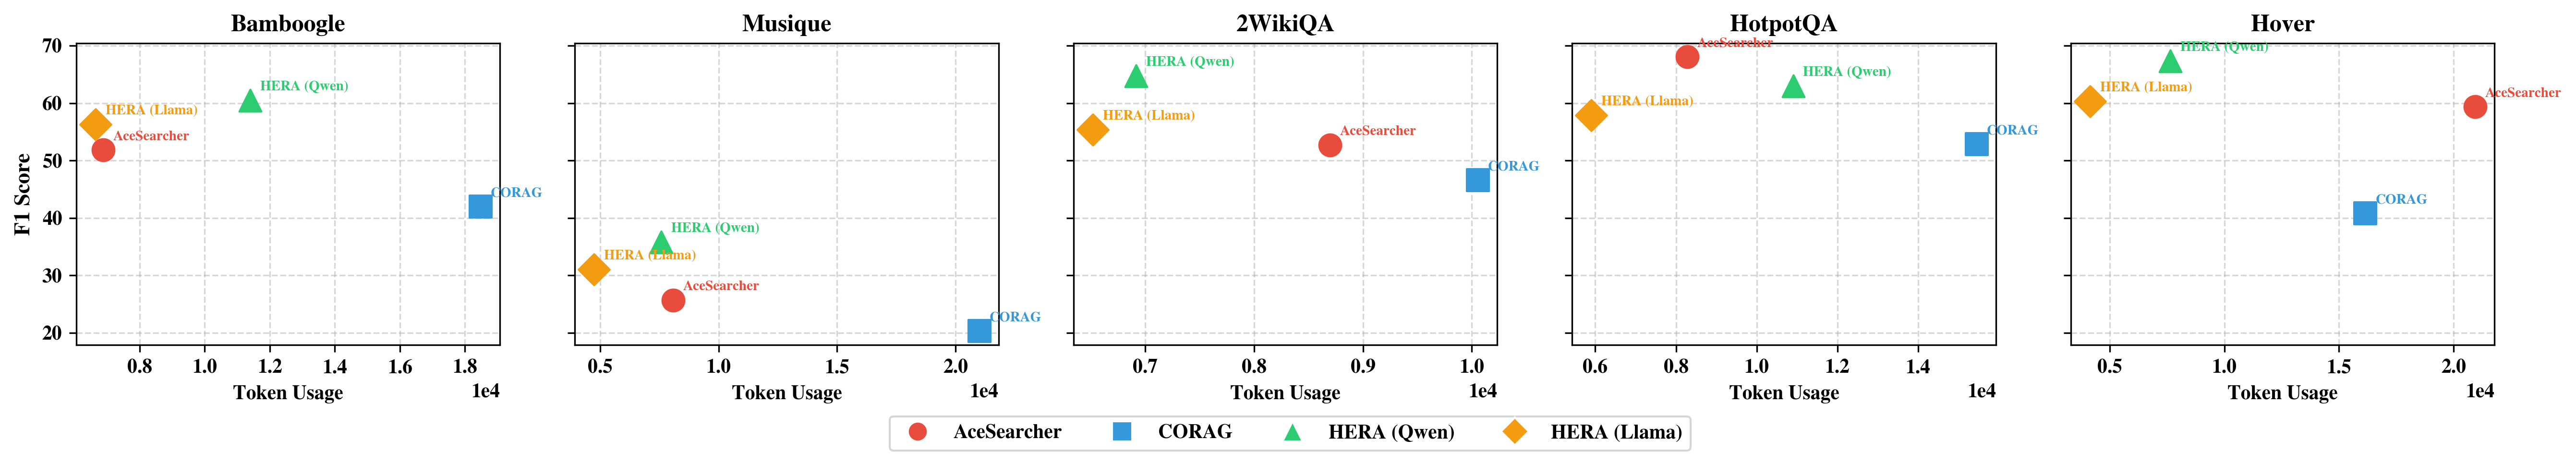
\includegraphics[width=1\linewidth]{figures/f1_vs_tokens.png}
        \vspace{-12pt}
        \caption{Comparison of Performance–Token Efficiency Trade-off with Selected Baselines.}
        \label{fig:f1_tokens}

    \end{figure}
\vspace{10pt}
Figure~\ref{fig:f1_tokens} compares multi-hop QA performance against token consumption. Key observations include: \textbf{(i) Superior Performance–Efficiency Trade-off}. Across all datasets, \hero consistently dominates the performance–efficiency frontier, achieving higher F1 scores with controlled token budgets. This demonstrates that gains arise from efficient reasoning trajectories instead of brute-force context scaling.
\textbf{(ii) Backbone-Specific Patterns.)} \hero with \qwen achieves the highest absolute performance, whereas \hero with \llama consistently minimizes token consumption ($\sim$4.7k–6.6k across most datasets) while preserving competitive F1 scores, indicating favorable computational efficiency. \textbf{(iii) Consistent performance and efficiency gains over baselines}.  CORAG uses the largest number of tokens across most datasets (up to $20k+$) without converting these costs into sustainable reasoning improvements or effective knowledge reuse, resulting in suboptimal F1 (\eg, 20.30 on MusiQue and 40.82 on HoVer). AceSearcher occupies an intermediate position, balancing moderate token usage and performance. 